\documentclass[11pt, a4paper]{article}

% ─── Packages ───
\usepackage[utf8]{inputenc}
\usepackage[T1]{fontenc}
\usepackage{lmodern}
\usepackage[margin=2.5cm]{geometry}
\usepackage{graphicx}
\usepackage{amsmath, amssymb}
\usepackage{booktabs}
\usepackage{multirow}
\usepackage{hyperref}
\usepackage{caption}
\usepackage{subcaption}
\usepackage{float}
\usepackage{enumitem}
\usepackage{xcolor}

\hypersetup{
    colorlinks=true,
    linkcolor=blue!70!black,
    citecolor=blue!70!black,
    urlcolor=blue!70!black
}

% ─── Title ───
\title{\textbf{Reinforcement Learning for the Snake Game:\\A Comparative Study of Value-Based and Policy Gradient Methods}}
\author{Gianluca Caregnato}
\date{}

\begin{document}
\maketitle

% ═══════════════════════════════════════════════════
% SECTION 1 — INTRODUCTION
% ═══════════════════════════════════════════════════
\section{Introduction}

The Snake game offers a deceptively simple setting for studying reinforcement learning: an agent
navigates a bounded grid, collects fruit to grow longer, and must avoid colliding with walls or
with its own body. Despite the straightforward rules, the problem poses several challenges that
make it a compelling testbed for RL algorithms. The state space is structured as a two-dimensional
grid, the reward signal is sparse, and---most critically---the environment provided for this project
is \emph{continuous}, meaning the game never terminates. There are no episode boundaries: the
snake persists indefinitely, wall collisions simply prevent movement, and self-collisions shorten
the tail rather than ending the game. This non-episodic nature forces a careful rethinking of
algorithms that typically assume well-defined episodes with terminal states.

In this work, we approach the problem from multiple angles. We first establish a
non-learning baseline using a \textbf{Greedy Breadth-First Search (BFS)} heuristic, which
deterministically follows the shortest path to the fruit. This baseline provides a principled
reference point: it achieves zero wall hits and a consistent average reward, but remains
fundamentally limited because it is purely reactive and does not reason about the long-term
consequences of the snake's growing body.

We then implement and compare three reinforcement learning algorithms of increasing
sophistication. \textbf{Deep Q-Network (DQN)} approximates the action-value function with a
neural network and learns from stored experience through off-policy updates.
\textbf{REINFORCE with baseline} directly optimizes the policy via Monte Carlo estimates of the
return, using a learned value function to reduce the variance of the gradient signal.
\textbf{Actor-Critic}, implemented as a bonus, combines a policy network (actor) with a value
network (critic) in a shared architecture, computing advantages from bootstrapped returns rather
than full Monte Carlo rollouts, which results in lower-variance updates at the cost of introducing
some bias.

All three agents share a common convolutional neural network backbone tailored to the grid
structure of the state, and all benefit from \emph{action masking}---a technique that prevents
the agent from selecting actions that would lead into a wall, effectively pruning clearly
suboptimal choices from the action space.

A key aspect of this study is the comparison between two environment settings:
\textbf{fully observable}, where the agent sees the entire $7 \times 7$ board, and
\textbf{partially observable}, where it only receives a local $5 \times 5$ window centered on the
snake's head. This comparison reveals how limited information impacts both the heuristic baseline
and the learned agents, and highlights the ability of RL methods to generalize under uncertainty.

The remainder of this report is organized as follows. Section~2 describes the environment in
detail and discusses the critical issues it poses for reinforcement learning.
Section~3 presents the Greedy BFS baseline and its adaptation to partial observability.
Section~4 covers the neural network architecture and the three RL algorithms, explaining every
design choice and its motivation. Section~5 reports the experimental results, including learning
curves and a final performance comparison. Section~6 concludes with a discussion of the
findings and possible directions for improvement.

% ═══════════════════════════════════════════════════
% SECTION 2 — ENVIRONMENT
% ═══════════════════════════════════════════════════
\section{Environment}

The game takes place on a $7 \times 7$ grid with walls on the border, leaving a $5 \times 5$
playable area containing one fruit and a snake (head + body). The environment runs $N$ boards
in parallel ($N{=}1000$ for training, $N{=}100$ for evaluation). Each cell is one-hot encoded
into 4 channels (\textsc{Empty}, \textsc{Fruit}, \textsc{Body}, \textsc{Head}), and the agent
chooses among four actions: Up, Right, Down, Left.

\paragraph{Rewards.}
Eating a fruit yields $+0.5$ and grows the snake by one segment. Hitting a wall gives $-0.1$
(the snake stays in place). Self-collision gives $-0.2$ and truncates the body from the
collision point to the tail---notably, the penalty is fixed regardless of how many segments are
lost. Normal steps yield $0$. Filling the entire board awards $+1.0$ and resets it, though this
event is exceedingly rare on a $5 \times 5$ grid.

\paragraph{Continuous environment.}
The game \textbf{never terminates}: there are no episode boundaries. This is the environment's
most critical property for algorithm design. DQN handles this naturally through single-step
bootstrapping. REINFORCE, however, requires an adaptation: since it is a Monte Carlo method
that assumes complete episodes, we collect fixed-length rollouts (50~steps) and bootstrap
$V(s_T)$ at the end to approximate the infinite-horizon return (Section~\ref{sec:reinforce}).
Actor-Critic uses $n$-step returns with bootstrapping by design ($n{=}5$), so no modification
is needed.

\paragraph{Observability.}
We evaluate two settings: \textbf{fully observable}, where the agent sees the entire
$7 \times 7$ board, and \textbf{partially observable}, where it receives only a $5 \times 5$
window centered on the head. In the latter, the fruit may be invisible, making the task
considerably harder.


% ═══════════════════════════════════════════════════
% SECTION 3 — BASELINE
% ═══════════════════════════════════════════════════
\section{Baseline: Greedy BFS Heuristic}

As a non-learning reference, we implement a greedy heuristic that uses \textbf{Breadth-First
Search} (BFS) to find the shortest path from the snake's head to the fruit, avoiding walls and
body segments. If the fruit is reachable, the agent takes the first action along the shortest
path; otherwise, it selects a random safe action (one that does not collide with a wall).

\paragraph{Action masking.}
All agents, including the baseline, benefit from \emph{action masking}: before selecting an
action, we check which of the four moves would immediately collide with a wall and exclude
them. For neural network agents, this is implemented by setting the logits of invalid actions to
$-\infty$ before the softmax (policy methods) or the argmax (DQN). This simple technique
eliminates all wall hits and narrows the effective action space.

\paragraph{Partial observability adaptation.}
For the partially observable setting, the baseline only has access to the $5 \times 5$ local
window around the head. If the fruit is visible within this window, BFS is applied on the local
view. If not, the agent takes a random safe action, since it has no information about the
fruit's location. This ``fair'' baseline ensures the comparison with RL agents is meaningful:
both the heuristic and the learned agents operate under the same information constraint.

% ═══════════════════════════════════════════════════
% SECTION 4 — METHODS
% ═══════════════════════════════════════════════════
\section{Methods}

All agents are implemented in \textbf{TensorFlow 2 / Keras}, which is the same framework used
by the environment. This eliminates inter-framework data conversion: the environment outputs
states in channels-last format \texttt{(N, H, W, 4)}, which Keras consumes directly.

\subsection{Shared CNN Backbone}

Since the state is a 2D grid, all agents share a convolutional backbone:
two \texttt{Conv2D} layers ($4 {\to} 32$ and $32 {\to} 64$ filters, $3 {\times} 3$ kernels,
padding \texttt{same}, ReLU activations) followed by a fully connected layer that compresses
the flattened feature maps into a 128-dimensional vector. This compact architecture is
appropriate for the small board size and avoids overfitting. Each algorithm attaches a different
head to this backbone: a Q-value head for DQN, a policy head for REINFORCE, or both a policy
and value head for Actor-Critic.

\subsection{Deep Q-Network (DQN)}

DQN approximates the action-value function $Q(s, a; \theta)$ with the CNN backbone plus a
two-layer head ($128 {\to} 64 {\to} 4$). The agent selects actions via an
$\varepsilon$-greedy policy: with probability
$\varepsilon = 0.05 + 0.95 \cdot e^{-t / 2000}$ it takes a random valid action, otherwise it
picks $\arg\max_a Q(s, a)$.

\paragraph{Experience replay.}
Transitions $(s, a, r, s')$ from all parallel boards are stored in a replay buffer of capacity
500\,000. At each training step, a mini-batch of 256 transitions is sampled uniformly at random.
This breaks temporal correlations and makes the training data approximately i.i.d., which is
essential for stable SGD convergence.

\paragraph{Target network and Double DQN.}
A target network $Q(s, a; \theta^-)$ provides stable TD targets. It is updated via Polyak
averaging ($\theta^- \leftarrow \tau\,\theta + (1{-}\tau)\,\theta^-$, $\tau{=}0.005$) every
200 training steps. We use the \textbf{Double DQN} variant to reduce overestimation bias:
the online network selects the best action, while the target network evaluates it:
\begin{equation}
y = r + \gamma \, Q\!\bigl(s',\, \arg\max_{a'} Q(s', a'; \theta);\, \theta^-\bigr).
\end{equation}
The loss is $\mathcal{L} = \text{MSE}(Q(s, a; \theta),\, y)$, optimized with Adam.

\subsection{REINFORCE with Baseline}
\label{sec:reinforce}

REINFORCE directly optimizes a stochastic policy $\pi(a|s; \theta)$ via the policy gradient
theorem. The policy head outputs a softmax distribution over actions (with invalid actions
masked to $-\infty$), and actions are sampled from this distribution during training.

\paragraph{Return computation with bootstrapping.}
For each training iteration, the agent collects a rollout of $T{=}50$ steps. Since the
environment is continuous (Section~2), we cannot set $G_T = 0$ at the rollout boundary.
Instead, we bootstrap:
\begin{equation}
G_T = V(s_T; w), \qquad G_t = r_t + \gamma \, G_{t+1} \quad \text{for } t = T{-}1, \ldots, 0,
\end{equation}
where $V(s; w)$ is a learned value network (the baseline). This value network has the same CNN
backbone but with a scalar output head ($128 {\to} 64 {\to} 1$).

\paragraph{Policy and value updates.}
The advantage $A_t = G_t - V(s_t; w)$ serves as a variance-reduced learning signal. The policy
is updated by ascending the gradient:
\begin{equation}
\nabla_\theta J \approx \frac{1}{TN} \sum_{t,n} \nabla_\theta \log \pi(a_t^{(n)} | s_t^{(n)}; \theta) \, A_t^{(n)},
\end{equation}
while the value network is trained to minimize $\text{MSE}(V(s_t), G_t)$. We apply return
whitening (standardizing returns to zero mean and unit variance) for training stability and
add an entropy bonus ($\beta{=}0.01$) to encourage exploration.

\subsection{Actor-Critic (Bonus)}

The Actor-Critic agent combines a policy (actor) and value function (critic) in a single
network with a shared CNN backbone and separate heads. This is more parameter-efficient
than REINFORCE, which uses two independent networks.

The key difference from REINFORCE is in the return estimation: instead of 50-step Monte Carlo
rollouts, Actor-Critic uses $n$-step returns ($n{=}5$) with bootstrapping:
\begin{equation}
G_t = r_t + \gamma r_{t+1} + \cdots + \gamma^{n-1} r_{t+n-1} + \gamma^n V(s_{t+n}; w).
\end{equation}
This introduces some bias compared to Monte Carlo but substantially reduces variance,
leading to more stable and data-efficient learning. The total loss combines the policy gradient
loss, a value prediction loss weighted by $0.5$, and the entropy bonus.

\subsection{Hyperparameters}

\begin{table}[H]
\centering
\small
\begin{tabular}{lccc}
\toprule
\textbf{Parameter} & \textbf{DQN} & \textbf{REINFORCE} & \textbf{Actor-Critic} \\
\midrule
Learning rate     & $5 \times 10^{-4}$ & $5 \times 10^{-4}$ (policy) / $1.5 \times 10^{-3}$ (value) & $5 \times 10^{-4}$ \\
Discount $\gamma$ & 0.95 & 0.95 & 0.95 \\
Batch / rollout   & 256 & 50 steps & 5 steps \\
$\varepsilon$ decay & 2\,000 steps & --- & --- \\
Entropy coeff.    & --- & 0.01 & 0.01 \\
Training iters    & 100\,000 & 10\,000 & 10\,000 \\
Parallel boards   & 1\,000 & 200 & 1\,000 \\
\bottomrule
\end{tabular}
\caption{Hyperparameter configuration for each algorithm.}
\label{tab:hyperparams}
\end{table}


% ═══════════════════════════════════════════════════
% SECTION 5 — RESULTS
% ═══════════════════════════════════════════════════
\section{Experimental Results}

All agents are evaluated on 100 parallel boards for 1\,000 steps with seed 0, using greedy
action selection (no exploration). Table~\ref{tab:results} reports the main metrics.

\begin{table}[H]
\centering
\small
\begin{tabular}{llcccc}
\toprule
\textbf{Environment} & \textbf{Agent} & \textbf{Avg Reward} & \textbf{Fruits} & \textbf{Self Hits} & \textbf{Wall Hits} \\
\midrule
\multirow{4}{*}{Fully Obs.}
 & Baseline (BFS) & 0.1124 & 23\,484 & 2\,516 & 0 \\
 & DQN            & \textbf{0.1368} & \textbf{29\,156} & 4\,477 & 0 \\
 & REINFORCE      & 0.1308 & 28\,774 & 6\,514 & 0 \\
 & Actor-Critic   & 0.1307 & 28\,848 & 6\,777 & 0 \\
\midrule
\multirow{4}{*}{Partial Obs.}
 & Baseline (BFS) & 0.0878 & 18\,475 & 2\,280 & 0 \\
 & DQN            & \textbf{0.1234} & \textbf{26\,419} & 4\,346 & 0 \\
 & REINFORCE      & 0.1173 & 25\,691 & 5\,559 & 0 \\
 & Actor-Critic   & 0.1193 & 26\,116 & 5\,646 & 0 \\
\bottomrule
\end{tabular}
\caption{Evaluation results (100 boards, 1\,000 steps, seed 0). Best values per environment
in bold.}
\label{tab:results}
\end{table}

\paragraph{All RL agents surpass the baseline.}
In the fully observable setting, DQN achieves the highest average reward (0.1368), followed
by REINFORCE (0.1308) and Actor-Critic (0.1307). All three exceed the BFS baseline
(0.1124) by 16--22\%. The advantage of RL agents stems from their ability to learn long-term
strategies---the baseline is purely reactive and makes no effort to avoid future self-collisions.

\paragraph{Partial observability degrades all agents.}
The baseline drops from 0.1124 to 0.0878 ($-22\%$) because it can no longer always locate the
fruit. RL agents show a smaller degradation ($\approx\!10\%$ for DQN), demonstrating that
neural networks learn implicit exploration strategies even with limited vision.

\paragraph{Self-collision trade-off.}
RL agents eat significantly more fruit than the baseline but also suffer more self-collisions.
REINFORCE and Actor-Critic have the highest self-hit rates (6\,500+), which correlates with
their slightly lower rewards. DQN achieves the best balance between fruit collection and
self-avoidance, with the fewest self-hits among all RL agents.

\paragraph{Learning curves.}
Figure~\ref{fig:learning_curves} shows the training reward over iterations. DQN converges
slowly but steadily over 100\,000 iterations. REINFORCE and Actor-Critic reach comparable
performance in only 10\,000 iterations, though with higher variance.

\begin{figure}[H]
\centering
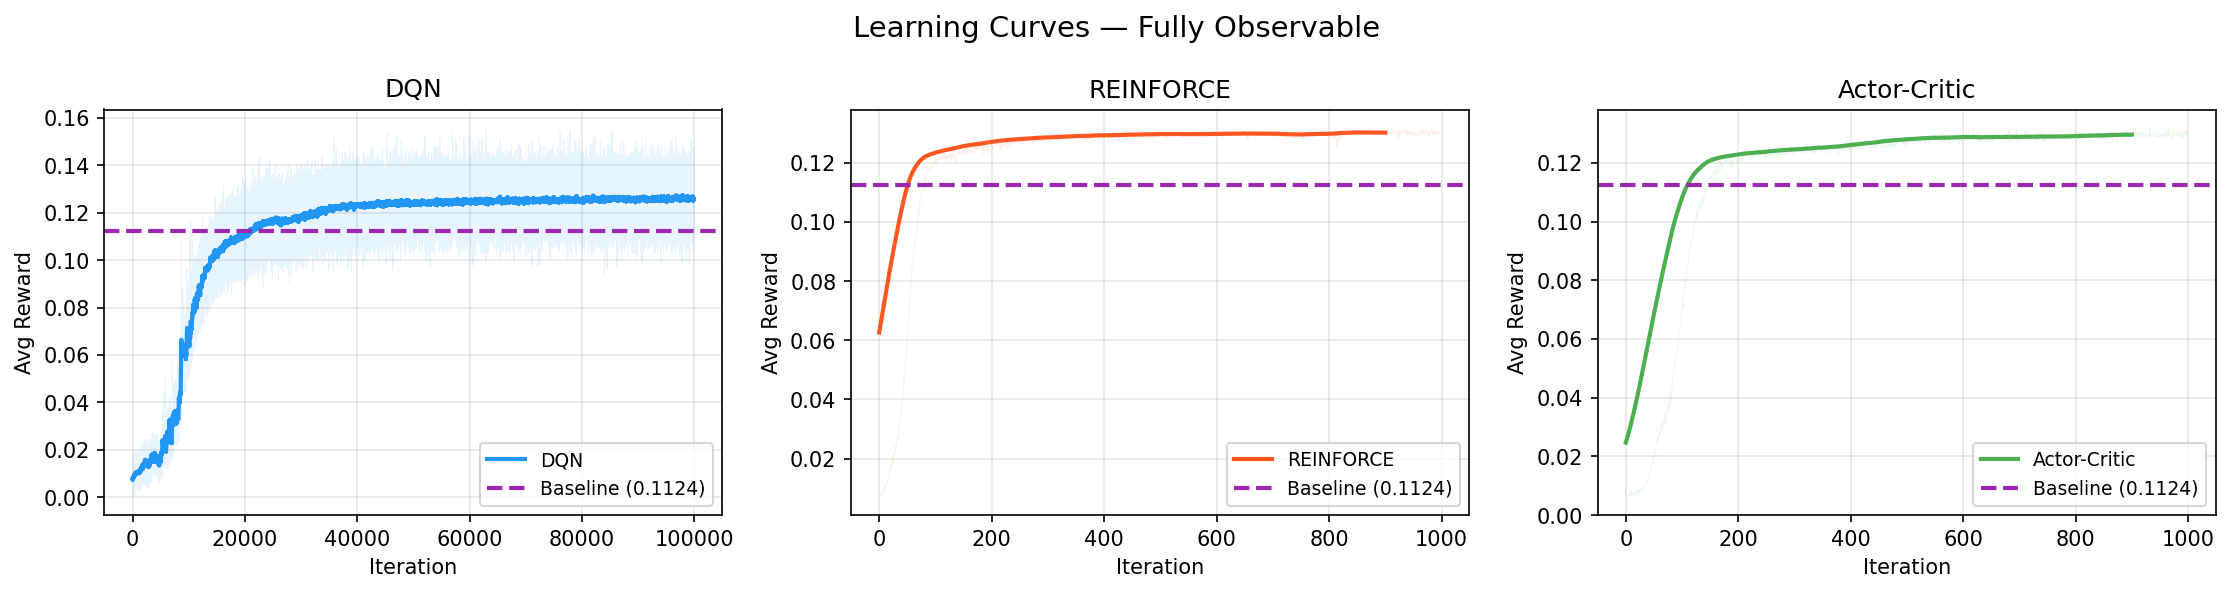
\includegraphics[width=\textwidth]{figures/learning_curves_fully_observable.png}
\caption{Learning curves for the fully observable environment (smoothed with a 100-step
moving average). The dashed line indicates the BFS baseline reward.}
\label{fig:learning_curves}
\end{figure}

\begin{figure}[H]
\centering
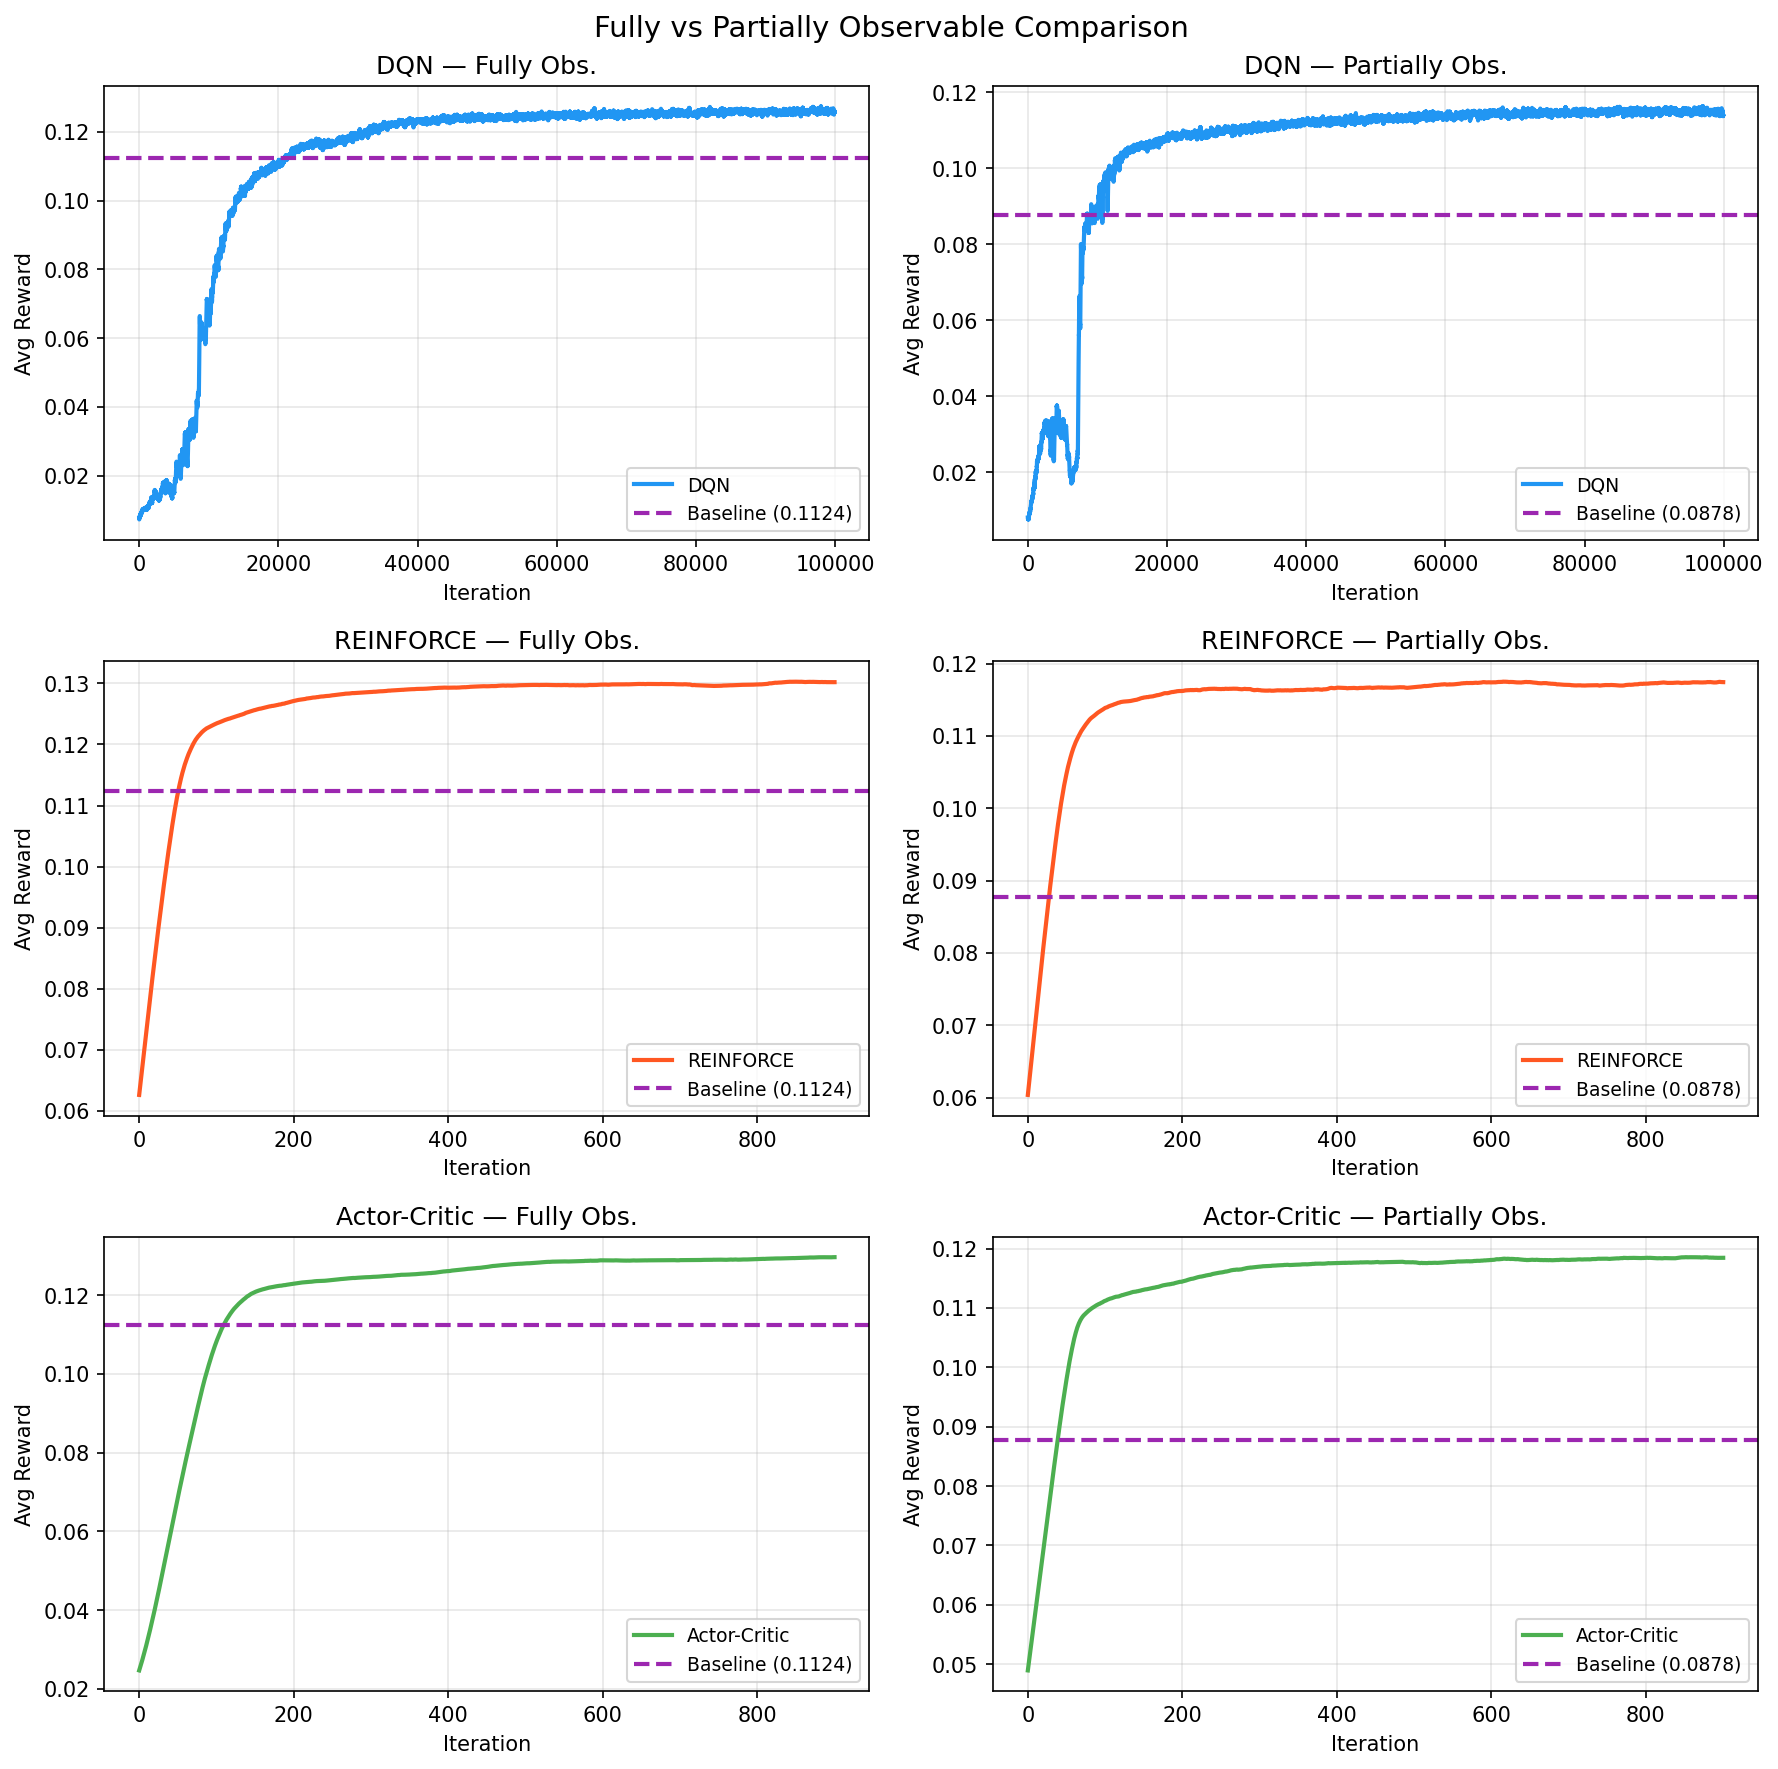
\includegraphics[width=\textwidth]{figures/comparison_observability.png}
\caption{Learning curves comparison between fully and partially observable environments.}
\label{fig:comparison}
\end{figure}

% ═══════════════════════════════════════════════════
% SECTION 6 — CONCLUSION
% ═══════════════════════════════════════════════════
\section{Conclusion}

We compared three reinforcement learning algorithms---DQN, REINFORCE with baseline, and
Actor-Critic---on the Snake environment, benchmarking them against a Greedy BFS heuristic in
both fully and partially observable settings.

All three RL agents consistently outperform the reactive baseline, confirming that learned
policies can capture long-term strategic reasoning that hand-crafted heuristics miss. DQN
achieves the best results in both settings, while REINFORCE and Actor-Critic perform similarly
but suffer from higher self-collision rates. The continuous (non-episodic) nature of the
environment posed a key challenge for REINFORCE, requiring a bootstrapping adaptation that
bridges the gap between Monte Carlo methods and temporal-difference learning.

Partial observability reduces all agents' performance, but RL methods are affected less than the
baseline ($\approx\!9\%$ vs.\ $22\%$ degradation). This suggests that neural network policies
learn to compensate for missing information through implicit exploration, whereas the BFS
baseline simply fails when the fruit is out of view.

\paragraph{Future work.}
Several directions could improve performance further:
\emph{(i)}~reward shaping, such as adding a small distance-to-fruit bonus for denser
supervision;
\emph{(ii)}~recurrent architectures (e.g., LSTM) for partial observability, enabling the agent
to remember previously seen fruit positions;
\emph{(iii)}~curriculum learning, starting on a larger board and gradually reducing it to
encourage robust policies.


\end{document}
